% capitulo de implementación
\chapter{Diseño e Implementación}
\section{Arquitectura de la solución}
El siguiente capitulo consta de las bases necesarias para realizar la solución. Esta se compone de 2 elementos principales. 
\begin{itemize}
\item Servidor: Encargado de recodificar (si es necesario) la fuente de audio o video y segmentarla para su distribución.
\item Cliente: Aplicación ejecutada en iOS, encargada de comunicarse al servidor para pedir el flujo de video y entregar información en twitter.
\end{itemize}
% poner figura aqui
La figura \ref{diagramaGral} presenta una idea general del sistema.\\

\begin{figure}[h!]
	\centering
	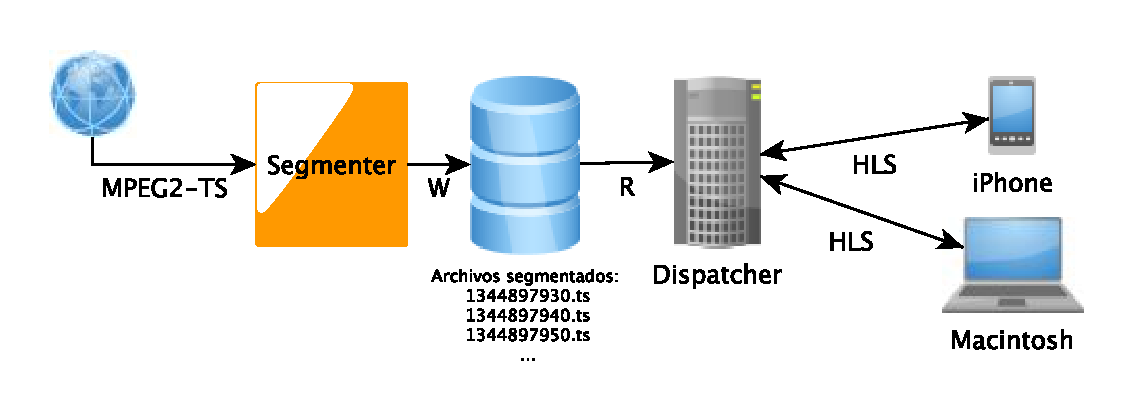
\includegraphics[scale=0.8]{imgs/diagrama_general.eps}
	\caption{Diagrama general de la solución}
	\label{diagramaGral}	
\end{figure}

Respecto a los elementos principales, estos se componen de distintos modulos que serán explicados con más detalle a lo largo del capítulo. Del diagrama se explican de forma general:
\begin{itemize}
\item Segmenter: es una aplicacion que recibe como entrada un flujo de audio y/o video encapsulado en MPEG2-Transport Stream, para luego segmentar el contenido en archivos segmentados de menor duración, estos se guardan en el sistema de archivos del servidor.
\item Dispatcher: Este es un programa dedicado a recibir peticiones de los clientes, para entregar un flujo de video mediante el protocolo HTTP Live Streaming.
\item iPhone y Macintosh: Son los dispositivos clientes controlados por el usuario, en estos se realiza el intercambio de ordenes para recibir el flujo de video que se quiere ver.
\end{itemize}

\subsection{Requerimiento Obligatorio}
% https://developer.apple.com/news/index.php?id=02162010a
	El protocolo utilizado para entregar el contenido audiovisual es HTTP Live Streaming (HLS). Los motivos de esta elección se deben a requerimientos obligatorios designados por Apple para la distribución de contenidos multimedia para su sistema operativo iOS.\\
	
	En un anuncio realizado por Apple en su sitio web destinado a desarrolladores, indica como obligación que la entrega de contenido del tipo audio y/o video con una una duración mayor a 10 minutos debe utilizar el protocolo HTTP Live Streaming, ya sea el enlace mediante WiFi o red celular. Además las aplicaciones deben incluir un flujo de datos (stream) de baja calidad con una cadencia de datos no superior a 64 kilobits/segundo, de manera que estas aplicaciones mantengan fluidez de conteido a pesar de encontrarse en condiciones desfavorables en la red.
	
	En caso de no seguir esta indicación, el desarrollador arriesga que su aplicación no sea admitida en la plataforma principal para la distribución de aplicaciones: iTunes Store.

	Considerando que este trabajo de memoria busca incorporar a los dispositivos iOS como consumidores del contenido multimedia utilizando timeshift, se debió diseñar la solucion alrededor de este protocolo.

%en resumen un acercamiento a como funciona la cosa

%\part{Primera parte}
\section{Protocolo HTTP Live Stream}
% https://developer.apple.com/resources/http-streaming/
% http://en.wikipedia.org/wiki/HTTP_Live_Streaming
% http://en.wikipedia.org/wiki/Progressive_download
% http://en.wikipedia.org/wiki/HyperText_Transfer_Protocol

El protocolo HTTP Live Streaming o HLS (abreviado), es un protocolo desarrollado por Apple Inc. para la distribución de multimedia a través de redes de computadores, de manera que el usuario consume el producto a medida que se descarga, es decir de forma continua.\\

Su carácteristica principal es la utilización del protocolo para transferencias de hipertexto, HTTP (hypertext transfer protocol) por sus siglas en inglés. Si bien HTTP se diseño originalmente para la World Wide Web como vía de entrega del texto en formato HTML, este se puede utilzar para distribuir datos de otros formatos codificados para habilitar su distribución.\\

HLS funciona entregando el contenido de forma segmentada al cliente, el cual tiene la responsabilidad de manejar la lógica de cambio de segmentos. Para distribuir el contenido se codifica la fuente de audio y/o video en varios archivos de corta duración, recomendandose entre 5 y 10 segundos, y que pueden o no tener el mismo bitrate. Estos pequeños archivos se ordenan en una lista de reproducción de formato .M3U8 que se entrega al reproductor del cliente. \\
También existe una variante donde la lista de reproducción contiene referencias a otras listas de reproducción con otras variantes de flujos de datos. \\

% http://www.streamingmedia.com/Articles/Editorial/What-Is-.../What-is-HLS-(HTTP-Live-Streaming)-78221.aspx
% In the Apple App Store, if you produce an app that delivers video longer then ten minutes or greater than 5MB of data, you must use  HTTP Live Streaming, and provide at least one stream at 64Kbps or lower bandwidth. Any streaming publisher targeting iOS devices via a website or app should know the basics of HLS and how it’s implemented.
	\subsection{Especificación}
		El protocolo HLS consiste en ordenar la entrega de archivos discretos a través de HTTP.
		El procedimiento general consiste en segmentar el contenido multimedia (audio y/o video) en pequeños archivos de manera que a través de un servidor web regular el cliente pueda descargar y unir los segmentos para verlos de manera continua. Esta forma de entregar el contenido puede ser utilizada para contenido pre-grabado o en vivo, difiriendo levemente en el componente encargado de ordenar los segmentos.\\
		

\clearpage		
\begin{figure}[h!]
	\centering
	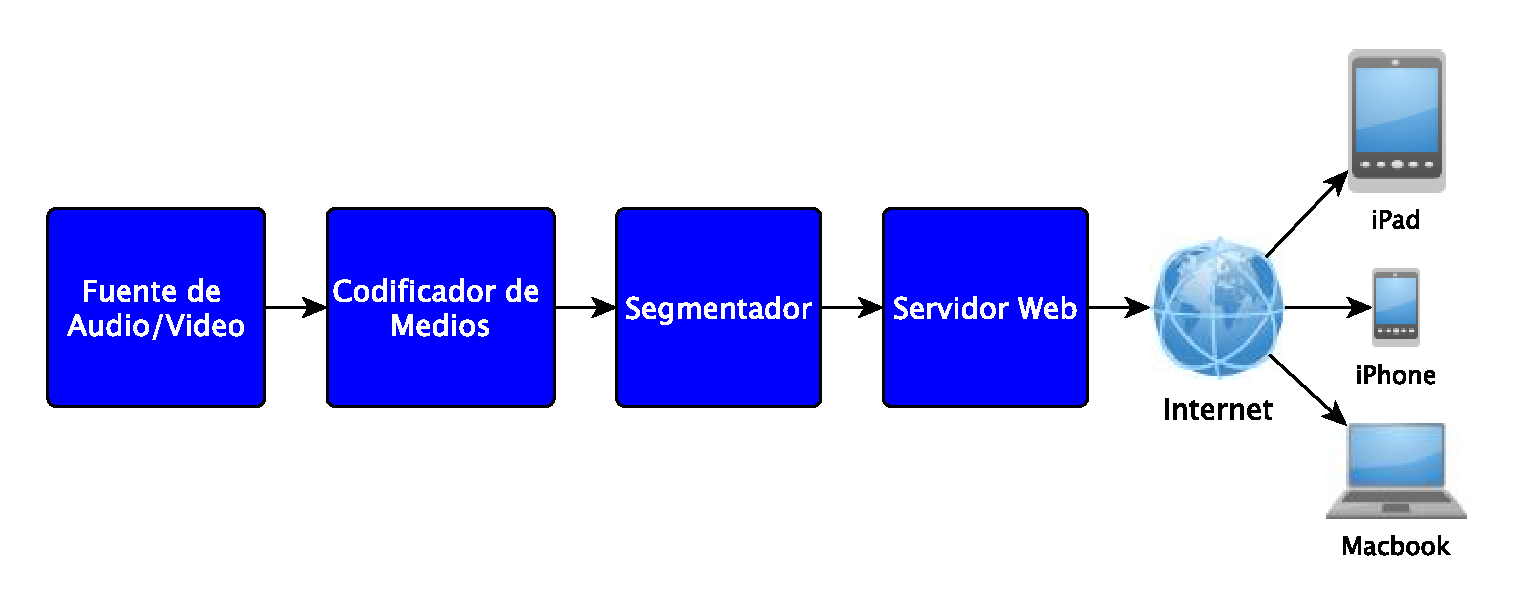
\includegraphics[scale=0.5]{imgs/HLS_diagram_wwdc2010.eps}
	\caption{Flujo de trabajo de HTTP Live Streaming}
	\label{diagramaHLSwwdc2010}	
\end{figure}		
		La figura \ref{diagramaHLSwwdc2010} presenta un ejemplo de distribucion de multimedia a través de HTTP Live Streaming.\\
		
En primera instancia se debe obtener contenido multimedia ya sea en un archivo fijo o flujo de datos, este contenido debe ser codificado para que sea compatible con los dispositivos que corren iOS, generalmente por recomendación de Apple se deben utilizar los codec de video h.264 y de audio AAC (advanced audio coding). El empaquetado de este contenido ya codificado debe ser entregado a una aplicación encargada de segmentarlo en pequeños archivos. \\
	El flujo de transporte a utilizar es MPEG2-TS (MPEG2 Transport Stream), el resultado de la aplicación segmentadora es guardado en el sistema de archivos donde reside el servidor web (o una ubicación accesible) de manera que al recibir requerimientos de stream HLS, este pueda proveer una lista de reproducción en formato M3U8 que mantiene el orden de reproducción de los archivos.\\
	
Tomando en cuenta el funcionamiento del protocolo HLS, para distribuir el contenido multimedia generado en vivo se debe codificar y segmentar inmediatamente para que el servidor web pueda proveerlos. En el caso que el contenido es un gran archivo, la codificación y segmentación se realiza una sola vez.

\subsubsection{Lista de reproducción}

La lista de reproducción en formato M3U8 es lo entregado al cliente, este puede ser una aplición iOS o el navegador web Safari desarrollado por Apple. Esta lista consiste en enlaces (URL) absolutos o relativos de los segmentos siguiendo el orden del contenido. Además se incluyen comentarios precedidos por el caracter \textbf{\#}, en el caso que un comentario utilice una palabra conocida del protocolo se le denomina entonces como marca (tag).
Las marcas primordiales para una trasmision a través de HLS son las siguientes:

\begin{prop}

\item \#EXTM3U: Es la primera marca que inicia una lista de reproducción, siempre debe estar al principio.

\item \#EXT-X-TARGETDURATION: Esta marca corresponde a la mayor duración que puede poseer cualquier segmento, es decir los segmentos enumerados en la lista no pasarán del tiempo especificado por esta marca.
Además este valor indica al cliente cada cuanto tiempo debe realizar una petición al servidor web por la lista.
\label{TAG-targetduration}	

\item \#EXT-X-MEDIASEQUENCE: Corresponde a la versión de la lista de reproducción segun los segmentos incluidos en la lista de reproducción.

\item \#EXTINF: Esta marca indica la duración del segmento que se encuentra junto a él.\\
\end{prop}

\begin{figure}[h!]
	\centering
	\begin{lstlisting}
	#EXTM3U
	#EXT-X-TARGETDURATION:10
	#EXT-X-MEDIA-SEQUENCE:1
	#EXTINF:10,
	http://media.ejemplo.com/segmento0.ts
	#EXTINF:10,
	http://media.ejemplo.com/segmento1.ts
	#EXTINF:10,
	http://media.ejemplo.com/segmento2.ts
	#EXT-X-ENDLIST
	\end{lstlisting}
	\caption{Lista de reproducción del tipo Video-on-Demand}
	\label{ejemploM3U8}	
\end{figure}			

El ejemplo visto en la figura \ref{ejemploM3U8} destaca una marca extra: \#EXT-X-ENDLIST, la cual indica al cliente que la lista de reproducción está completa y no necesita ser actualizada. Esta marca toma gran importancia al definir un flujo de medios ``en vivo'' ya que al estar ausente el cliente pedirá una nueva versión de la lista de reproducción que incluya nuevos segmentos, el tiempo que indica la actualización depende de la marca \ref{TAG-targetduration} previamente explicada.

		% mostrar figura de playlist, explicacion rapida de como funciona hls
		\subsubsection{Draft Apple}
		% aqui detallar los mensajes de la playlist utilizados
		%		http://tools.ietf.org/html/draft-pantos-http-live-streaming-08
		\subsubsection{Caracteristicas a utilizar}
		% caracteristicas bacanes de hls, detallar lo que se puede hacer más aun
			
	\subsection{Herramientas dispuestas por Apple}
		\subsubsection{id3Tag Generator}
		\subsubsection{MediaStream Segmenter}
		\subsubsection{MediaFile Segmenter}
	\subsection{Ejemplo de transmisión}
	% explicar como se probó con resident evil y motorstorm
\clearpage	
\section{Reproducción y Control de Stream de Video}
	
	\subsection{Servidor HTTP}
		\subsubsection{Obtención del Stream}	
		\subsubsection{Sementación del Video}
		\subsubsection{Playlist Dispatcher}
	\subsection{Cliente iOS}
		\subsubsection{Recopilación de datos del Stream}
		\subsubsection{Reproducción con AV Framework}
	\subsection{Intercambio de información entre componentes}
\clearpage
\section{Interfaz Gráfica}
	\subsection{Apple Design Guidelines}
	\subsection{Componentes de UIKit}
		\subsubsection{UIDatePicker}
		\subsubsection{UIButton}
		\subsubsection{...etc}
\clearpage
\section{Integración Redes Sociales}
	\subsection{Twitter}
		\subsubsection{API Twitter}
		\subsubsection{Sharekit vs. Twitter Framework}
		\subsubsection{Post en Twitter}
		\subsubsection{Seguimiento de Hashtag}
		\subsubsection{Extracción de información de un Tweet}
	\subsection{Bit.ly}
		\subsubsection{API Bit.ly}
		\subsubsection{Seguimiento de un Hipervínculo}
		\subsubsection{Expansión de atajo bit.ly}
\clearpage
\section{Registro en iOS}
	\subsection{Schemes}
	\subsection{Redireccionamiento via Web}
		\subsubsection{PHP Script}
		\subsubsection{Respuestas según User Agent}